\section{Execution Stage}
In this stage, the most significant component to verify is the ALU with its internal operators. Initially,
two small testbenches were described to quickly test the adder and the barrel shifter (\texttt{tb\_adder} and
\texttt{tb\_barrelShifter}), mostly to check if they compiled and if they produced some results, meaning no signals
were left unassigned nor were they driven by multiple sources. When \texttt{tb\_ALU}, a more functional and flexible
testbench was realized, they were discarded and all the testbenches happened at the ALU datapath level.

The testbench process is composed of the following parts:
\begin{itemize}
    \item A Python script that generates meaningful inputs for an ALU with a specific file format
    \item A C++ description of the same ALU that generates the reference results
    \item A VHDL testbench that simulates the hardware behavior
\end{itemize}
The reference and the simulation results can then be compared to each other to complete the test.

\subsection{Input generation}
\label{sec:tb-input-gen}
Inputs are generated through a very simple Python script, that generates a certain number of inputs (specified by
command line) using the random number generators. Each line of the
generated output contains the following fields separated by spaces:
\begin{enumerate}
    \item 8 hex digits for operand 1
    \item 8 hex digits for operand 2
    \item 1 hex digit for the ALU opcode
\end{enumerate}
which are all the inputs of an ALU. Since, in VHDL, the ALU opcode is an enumeration that may be changed for
optimizations or various design reasons, the numbers that represent the various operations are arbitary and the
VHDL testbench will need a specific unit to convert the arbitrary signals into the ones that the circuit actually uses.
For example, the following line from a generated input file will represent an addition between 00000001 and
\texttt{ffffffff}.
\begin{lstlisting}
    00000001 ffffffff 0
\end{lstlisting}

\subsection{VHDL infrastructure}
This testbench instantiates a whole ALU, provides data and control inputs and stores the outputs. At the same time, it
instantiates a clock generator, an ALUFileReader and an ALUFileWriter.

\begin{figure}[htbp]
    \center
	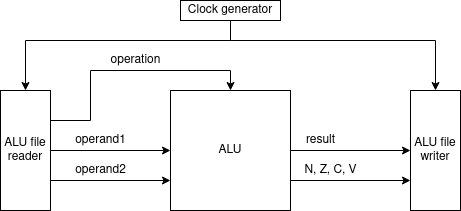
\includegraphics[width=0.6\textwidth]{./3-verification/images/tb_ALU.png}
	\caption{Structure of the testbench for ALU}
	\label{fig:tb-alu}
\end{figure}

As stated in \autoref{sec:tb-input-gen}, ALUFileReader has to map the arbitrary opcodes into the local enumeration,
this task is done through a function, described in the global package, that uses a switch to return the correct result.

\subsection{C++ Reference}
The software version of the ALU used to generate is implemented with a single C++ class called ALU. The declaration of
this class, along with a brief description of its functionality, is visible in \autoref{appendix:simulated-alu}.

By default, the compiled executable works in streaming mode: it continuously reads inputs from the standard input,
performs the operations and prints the outputs to the standard out until the user interrupts the stream. This is useful
for quickly testing specific input combinations by hand through the command line. It is possible to redirect the inputs
or outputs from/to files to simulate arbitrarily large sequences of inputs.

\subsection{Running the simulations}
Operand specific simulations can be executed manually by generating input sequences to feed to the reference and
to the simulation. Complete ALU simulations, instead, were scripted to simplify the whole process.
It is possible to launch the script by simply specifying the amount of inputs and the automated process takes care of
initializing the environment, generating the inputs, running the simulations and cleaning up. To get a decent coverage
of the possible input combinations, plenty of simulations with input files whose size ranged from 50'000 to 100'000
lines each were launched over the span of multiple testing sessions.
